\documentclass{standalone}
\usepackage{tikz}
\usetikzlibrary{patterns, positioning}

\begin{document}
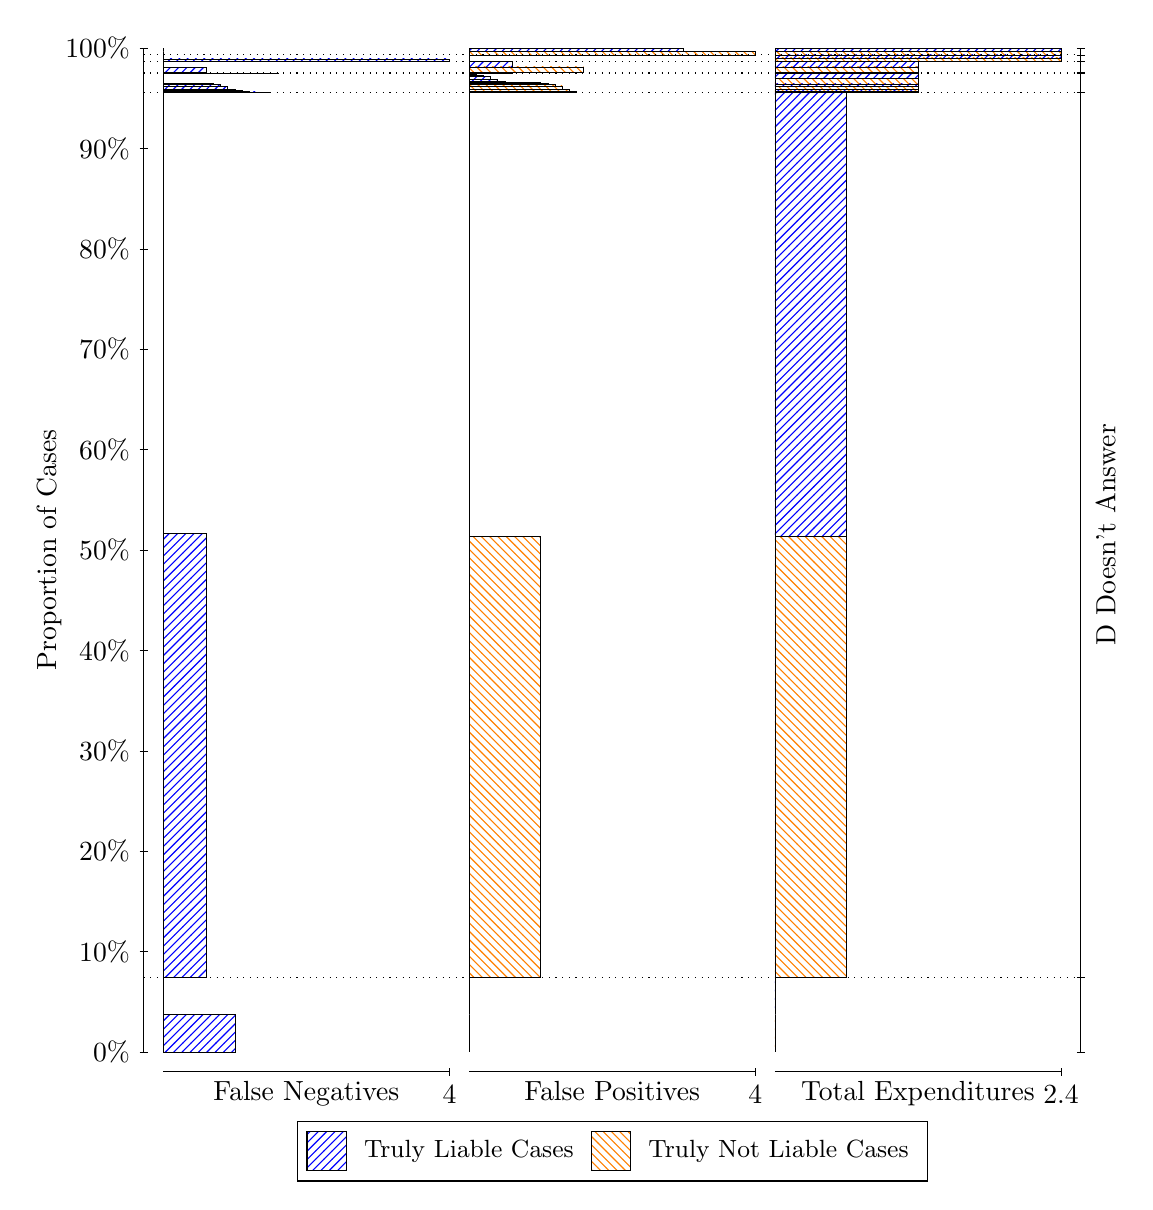
\begin{tikzpicture}
\draw[black, very thin] (1.5,1.75) -- (1.5,14.5);
\node[rotate=90, anchor=center] at (0.3, 8.125) {Proportion of Cases};
\draw[black, very thin] (1.45,1.75) -- (1.55,1.75);
\node[anchor=east] at (1.45, 1.75) {0\%};
\draw[black, very thin] (1.45,3.025) -- (1.55,3.025);
\node[anchor=east] at (1.45, 3.025) {10\%};
\draw[black, very thin] (1.45,4.3) -- (1.55,4.3);
\node[anchor=east] at (1.45, 4.3) {20\%};
\draw[black, very thin] (1.45,5.575) -- (1.55,5.575);
\node[anchor=east] at (1.45, 5.575) {30\%};
\draw[black, very thin] (1.45,6.85) -- (1.55,6.85);
\node[anchor=east] at (1.45, 6.85) {40\%};
\draw[black, very thin] (1.45,8.125) -- (1.55,8.125);
\node[anchor=east] at (1.45, 8.125) {50\%};
\draw[black, very thin] (1.45,9.4) -- (1.55,9.4);
\node[anchor=east] at (1.45, 9.4) {60\%};
\draw[black, very thin] (1.45,10.675) -- (1.55,10.675);
\node[anchor=east] at (1.45, 10.675) {70\%};
\draw[black, very thin] (1.45,11.95) -- (1.55,11.95);
\node[anchor=east] at (1.45, 11.95) {80\%};
\draw[black, very thin] (1.45,13.225) -- (1.55,13.225);
\node[anchor=east] at (1.45, 13.225) {90\%};
\draw[black, very thin] (1.45,14.5) -- (1.55,14.5);
\node[anchor=east] at (1.45, 14.5) {100\%};

\draw[black, very thin] (13.4,1.75) -- (13.4,14.5);
\draw[black, very thin] (13.35,1.75) -- (13.45,1.75);
\node[anchor=west] at (13.35, 1.75) {};
\draw[black, very thin] (13.35,2.699) -- (13.45,2.699);
\node[anchor=west] at (13.35, 2.699) {};
\draw[black, very thin] (13.35,13.936) -- (13.45,13.936);
\node[anchor=west] at (13.35, 13.936) {};
\draw[black, very thin] (13.35,14.178) -- (13.45,14.178);
\node[anchor=west] at (13.35, 14.178) {};
\draw[black, very thin] (13.35,14.186) -- (13.45,14.186);
\node[anchor=west] at (13.35, 14.186) {};
\draw[black, very thin] (13.35,14.326) -- (13.45,14.326);
\node[anchor=west] at (13.35, 14.326) {};
\draw[black, very thin] (13.35,14.414) -- (13.45,14.414);
\node[anchor=west] at (13.35, 14.414) {};
\draw[black, very thin] (13.35,14.5) -- (13.45,14.5);
\node[anchor=west] at (13.35, 14.5) {};

\draw[black, very thin, pattern color=blue, pattern=north east lines] (1.75,1.75) rectangle (2.6583,2.2245);
\draw[black, very thin, pattern color=orange, pattern=north west lines] (1.75,2.2245) rectangle (1.75,2.699);
\draw[black, very thin, pattern color=blue, pattern=north east lines] (1.75,2.699) rectangle (2.295,8.3364);
\draw[black, very thin, pattern color=orange, pattern=north west lines] (1.75,8.3364) rectangle (1.75,13.936);
\draw[black, very thin, pattern color=blue, pattern=north east lines] (1.75,13.936) rectangle (3.1125,13.937);
\draw[black, very thin, pattern color=blue, pattern=north east lines] (1.75,13.937) rectangle (3.0217,13.938);
\draw[black, very thin, pattern color=blue, pattern=north east lines] (1.75,13.938) rectangle (2.9308,13.942);
\draw[black, very thin, pattern color=blue, pattern=north east lines] (1.75,13.942) rectangle (2.84,13.945);
\draw[black, very thin, pattern color=blue, pattern=north east lines] (1.75,13.945) rectangle (2.7492,13.961);
\draw[black, very thin, pattern color=blue, pattern=north east lines] (1.75,13.961) rectangle (2.6583,13.977);
\draw[black, very thin, pattern color=blue, pattern=north east lines] (1.75,13.977) rectangle (2.5675,14.015);
\draw[black, very thin, pattern color=blue, pattern=north east lines] (1.75,14.015) rectangle (2.4767,14.039);
\draw[black, very thin, pattern color=blue, pattern=north east lines] (1.75,14.039) rectangle (2.3858,14.048);
\draw[black, very thin, pattern color=orange, pattern=north west lines] (1.75,14.048) rectangle (1.75,14.178);
\draw[black, very thin, pattern color=blue, pattern=north east lines] (1.75,14.178) rectangle (3.2033,14.182);
\draw[black, very thin, pattern color=orange, pattern=north west lines] (1.75,14.182) rectangle (1.75,14.186);
\draw[black, very thin, pattern color=blue, pattern=north east lines] (1.75,14.186) rectangle (2.295,14.251);
\draw[black, very thin, pattern color=orange, pattern=north west lines] (1.75,14.251) rectangle (1.75,14.326);
\draw[black, very thin, pattern color=blue, pattern=north east lines] (1.75,14.326) rectangle (5.3833,14.363);
\draw[black, very thin, pattern color=orange, pattern=north west lines] (1.75,14.363) rectangle (1.75,14.414);
\draw[black, very thin, pattern color=orange, pattern=north west lines] (1.75,14.414) rectangle (1.75,14.456);
\draw[black, very thin, pattern color=blue, pattern=north east lines] (1.75,14.456) rectangle (1.75,14.5);
\draw[black, very thin, pattern color=orange, pattern=north west lines] (5.6333,1.75) rectangle (5.6333,2.2245);
\draw[black, very thin, pattern color=blue, pattern=north east lines] (5.6333,2.2245) rectangle (5.6333,2.699);
\draw[black, very thin, pattern color=orange, pattern=north west lines] (5.6333,2.699) rectangle (6.5417,8.2985);
\draw[black, very thin, pattern color=blue, pattern=north east lines] (5.6333,8.2985) rectangle (5.6333,13.936);
\draw[black, very thin, pattern color=orange, pattern=north west lines] (5.6333,13.936) rectangle (6.9958,13.946);
\draw[black, very thin, pattern color=orange, pattern=north west lines] (5.6333,13.946) rectangle (6.905,13.974);
\draw[black, very thin, pattern color=orange, pattern=north west lines] (5.6333,13.974) rectangle (6.8142,14.018);
\draw[black, very thin, pattern color=orange, pattern=north west lines] (5.6333,14.018) rectangle (6.7233,14.036);
\draw[black, very thin, pattern color=orange, pattern=north west lines] (5.6333,14.036) rectangle (6.6325,14.055);
\draw[black, very thin, pattern color=orange, pattern=north west lines] (5.6333,14.055) rectangle (6.5417,14.059);
\draw[black, very thin, pattern color=orange, pattern=north west lines] (5.6333,14.059) rectangle (6.4508,14.063);
\draw[black, very thin, pattern color=orange, pattern=north west lines] (5.6333,14.063) rectangle (6.36,14.065);
\draw[black, very thin, pattern color=orange, pattern=north west lines] (5.6333,14.065) rectangle (6.2692,14.066);
\draw[black, very thin, pattern color=blue, pattern=north east lines] (5.6333,14.066) rectangle (6.0875,14.076);
\draw[black, very thin, pattern color=blue, pattern=north east lines] (5.6333,14.076) rectangle (5.9967,14.1);
\draw[black, very thin, pattern color=blue, pattern=north east lines] (5.6333,14.1) rectangle (5.9058,14.137);
\draw[black, very thin, pattern color=blue, pattern=north east lines] (5.6333,14.137) rectangle (5.815,14.153);
\draw[black, very thin, pattern color=blue, pattern=north east lines] (5.6333,14.153) rectangle (5.7242,14.17);
\draw[black, very thin, pattern color=blue, pattern=north east lines] (5.6333,14.17) rectangle (5.6333,14.178);
\draw[black, very thin, pattern color=orange, pattern=north west lines] (5.6333,14.178) rectangle (6.1783,14.182);
\draw[black, very thin, pattern color=blue, pattern=north east lines] (5.6333,14.182) rectangle (5.6333,14.186);
\draw[black, very thin, pattern color=orange, pattern=north west lines] (5.6333,14.186) rectangle (7.0867,14.26);
\draw[black, very thin, pattern color=blue, pattern=north east lines] (5.6333,14.26) rectangle (6.1783,14.326);
\draw[black, very thin, pattern color=orange, pattern=north west lines] (5.6333,14.326) rectangle (5.6333,14.376);
\draw[black, very thin, pattern color=blue, pattern=north east lines] (5.6333,14.376) rectangle (5.6333,14.414);
\draw[black, very thin, pattern color=orange, pattern=north west lines] (5.6333,14.414) rectangle (9.2667,14.456);
\draw[black, very thin, pattern color=blue, pattern=north east lines] (5.6333,14.456) rectangle (8.3583,14.5);
\draw[black, very thin, pattern color=orange, pattern=north west lines] (9.5167,1.75) rectangle (9.5167,2.2245);
\draw[black, very thin, pattern color=blue, pattern=north east lines] (9.5167,2.2245) rectangle (9.5167,2.699);
\draw[black, very thin, pattern color=orange, pattern=north west lines] (9.5167,2.699) rectangle (10.425,8.2985);
\draw[black, very thin, pattern color=blue, pattern=north east lines] (9.5167,8.2985) rectangle (10.425,13.936);
\draw[black, very thin, pattern color=orange, pattern=north west lines] (9.5167,13.936) rectangle (11.333,13.955);
\draw[black, very thin, pattern color=blue, pattern=north east lines] (9.5167,13.955) rectangle (11.333,13.972);
\draw[black, very thin, pattern color=orange, pattern=north west lines] (9.5167,13.972) rectangle (11.333,14.011);
\draw[black, very thin, pattern color=blue, pattern=north east lines] (9.5167,14.011) rectangle (11.333,14.045);
\draw[black, very thin, pattern color=orange, pattern=north west lines] (9.5167,14.045) rectangle (11.333,14.117);
\draw[black, very thin, pattern color=blue, pattern=north east lines] (9.5167,14.117) rectangle (11.333,14.178);
\draw[black, very thin, pattern color=orange, pattern=north west lines] (9.5167,14.178) rectangle (11.333,14.182);
\draw[black, very thin, pattern color=blue, pattern=north east lines] (9.5167,14.182) rectangle (11.333,14.186);
\draw[black, very thin, pattern color=orange, pattern=north west lines] (9.5167,14.186) rectangle (11.333,14.26);
\draw[black, very thin, pattern color=blue, pattern=north east lines] (9.5167,14.26) rectangle (11.333,14.326);
\draw[black, very thin, pattern color=orange, pattern=north west lines] (9.5167,14.326) rectangle (13.15,14.376);
\draw[black, very thin, pattern color=blue, pattern=north east lines] (9.5167,14.376) rectangle (13.15,14.414);
\draw[black, very thin, pattern color=orange, pattern=north west lines] (9.5167,14.414) rectangle (13.15,14.456);
\draw[black, very thin, pattern color=blue, pattern=north east lines] (9.5167,14.456) rectangle (13.15,14.5);
\draw[black, dotted] (1.5,2.699) -- (13.4,2.699);
\draw[black, dotted] (1.5,13.936) -- (13.4,13.936);
\draw[black, dotted] (1.5,14.178) -- (13.4,14.178);
\draw[black, dotted] (1.5,14.186) -- (13.4,14.186);
\draw[black, dotted] (1.5,14.326) -- (13.4,14.326);
\draw[black, dotted] (1.5,14.414) -- (13.4,14.414);
\draw[black, very thin] (1.75,1.5) -- (5.3833,1.5);
\node[anchor=north] at (3.5667, 1.5) {False Negatives};
\draw[black, very thin] (5.3833,1.45) -- (5.3833,1.55);
\node[anchor=north] at (5.3833, 1.45) {4};

\draw[black, very thin] (5.6333,1.5) -- (9.2667,1.5);
\node[anchor=north] at (7.45, 1.5) {False Positives};
\draw[black, very thin] (9.2667,1.45) -- (9.2667,1.55);
\node[anchor=north] at (9.2667, 1.45) {4};

\draw[black, very thin] (9.5167,1.5) -- (13.15,1.5);
\node[anchor=north] at (11.333, 1.5) {Total Expenditures};
\draw[black, very thin] (13.15,1.45) -- (13.15,1.55);
\node[anchor=north] at (13.15, 1.45) {2.4};


\node[black, centered, rotate=90] at (13.72, 8.3174) {D Doesn't Answer};






\draw (7.449999999999999,1.5) node[draw=none] (baseCoordinate) {};
\begin{scope}[align=center]
        \matrix[scale=0.5, draw=black, below=0.5cm of baseCoordinate, nodes={draw}, column sep=0.1cm]{
            \node[rectangle, draw, minimum width=0.5cm, minimum height=0.5cm, pattern=north east lines, pattern color=blue] {}; &
            \node[draw=none, font=\small] (B) {Truly Liable Cases}; &
            \node[rectangle, draw, minimum width=0.5cm, minimum height=0.5cm, pattern=north west lines, pattern color=orange] {}; &
            \node[draw=none, font=\small] (B) {Truly Not Liable Cases}; \\
            };
\end{scope}

\end{tikzpicture}
\end{document}